% !TeX encoding = UTF-8

\documentclass{protokol}


\usepackage{tikz}
\usetikzlibrary{calc}
\usetikzlibrary{arrows}

%====== Units =====
\usepackage{siunitx}
\sisetup{inter-unit-product =\ensuremath{\cdot}}
\sisetup{group-digits = integer}
\sisetup{output-decimal-marker = {,}}
\sisetup{exponent-product = \ensuremath{\cdot}}
\sisetup{separate-uncertainty}
\sisetup{tight-spacing = false}
%\sisetup{scientific-notation = true}
%\sisetup{round-mode=places,round-precision=4}
%\sisetup{evaluate-expression}


%====== Grafy =====
\usepackage{pgfplots}
\pgfplotsset{width=0.8\linewidth, compat=1.17}
\def\plotcscale{0.8}
\usepackage{pgfplotstable}
\usepackage[figurename=Obr.]{caption} % figure caption rename

%====== Rovnice align block ======
\usepackage{amsmath}
\setlength{\jot}{10pt} % rozestup mezi řádky

\graphicspath{ {./img/} }

%====== Vyplňte údaje ======
\jmeno{Jakub Charvot}
\kod{240844}
\rocnik{3.}
\obor{MET}
\skupina{MET/2}
\spolupracoval{--}

\merenodne{--}
\odevzdanodne{2.5.\ 2023}
\nazev{Vlastnosti materiálů tlustých vrstev}
\cislo{2} %měřené úlohy

\predmet{Mikroelektronika a technologie součástek}
\ustav{Ústav mikroelektroniky}
\skola{FEKT VUT v~Brně}

\def\para{x+0}
\def\parb{\para-80}


%citace 
% \usepackage[backend=biber, style=iso-numeric, sortlocale=cs_CZ, autolang=other, language=czech]{biblatex}
% \addbibresource{bibliography.bib}
% \DeclareFieldFormat{labelnumberwidth}{\mkbibbrackets{#1}}
% hyperlinky
\usepackage[colorlinks]{hyperref}

% odstavce
\usepackage{parskip}

% Bloky kódu
\usepackage{xcolor}

%New colors defined below
\definecolor{codegreen}{rgb}{0,0.6,0}
\definecolor{codegray}{rgb}{0.5,0.5,0.5}
\definecolor{codepurple}{rgb}{0.58,0,0.82}
\definecolor{backcolour}{rgb}{0.95,0.95,0.92}

\usepackage{listings}
\lstdefinestyle{mystyle}{
  backgroundcolor=\color{backcolour}, commentstyle=\color{codegreen},
  keywordstyle=\color{magenta},
  numberstyle=\tiny\color{codegray},
  stringstyle=\color{codepurple},
  basicstyle=\ttfamily\footnotesize,
  breakatwhitespace=false,         
  breaklines=true,                 
  captionpos=b,                    
  keepspaces=true,                 
  numbers=left,                    
  numbersep=5pt,                  
  showspaces=false,                
  showstringspaces=false,
  showtabs=false,                  
  tabsize=2
}
\lstset{
	inputencoding=utf8,
	extendedchars=true,
	literate={á}{{\'a}}1 {č}{{\v{c}}}1 {ď}{{\v{d}}}1 {é}{{\'e}}1 {ě}{{\v{e}}}1 
           {í}{{\'i}}1 {ň}{{\v{n}}}1 {ó}{{\'o}}1 {ř}{{\v{r}}}1 {š}{{\v{s}}}1 
           {ť}{{\v{t}}}1 {ú}{{\'u}}1 {ů}{{\r{u}}}1 {ý}{{\'y}}1 {ž}{{\v{z}}}1 
           {Á}{{\'A}}1 {Č}{{\v{C}}}1 {Ď}{{\v{D}}}1 {É}{{\'E}}1 {Ě}{{\v{E}}}1 
           {Í}{{\'I}}1 {Ň}{{\v{N}}}1 {Ó}{{\'O}}1 {Ř}{{\v{R}}}1 {Š}{{\v{S}}}1 
           {Ť}{{\v{T}}}1 {Ú}{{\'U}}1 {Ů}{{\r{U}}}1 {Ý}{{\'Y}}1 {Ž}{{\v{Z}}}1,
	style=mystyle
	}

% Číslování
\pagenumbering{arabic}



% =========================================
% =============== DOKUMENT ================
% =========================================
\begin{document}
	%====== Vygenerování tabulky ======
	\maketitle

\section{Teoretický úvod}
  Při použití tlustovrstvé technologie je potřeba uvědomit si faktory, které ovlivňují výslednou kvalitu a spolehlivost. Těchto faktorů je mnoho a odvíjí se zejména od použité technologie. 
  Např. při sítotisku musíme vzít v potaz parametry zvolené pasty, substrátu, na který nanášíme, a v neposlední řadě také samotného síta. Optimálního výsledku dosáhneme pouze vhodnou kombinací všech zmíněných faktorů. 

  Dnešní práce se věnuje vlastnotem používaných past. 
  
  \subsection{Reologické vlastnosti}
  Reologie je nauka o tomu a plynutí materiálů. Pro obecný popis tekutosti materiálu můžeme využít tzv. Debořino číslo T:
  \[
    T=  \frac{T_{rel}}{T_{obs} }
  \]
  kde \(T_{rel} \) je relaxační doba daného materiálu a \(T_{obs} \) je doba pozorování.
	
  \subsubsection{Viskozita}
    Viskozita popisuje vnitřní tření kapalin, to ovšem není konstantní, naopak je závislé na několika faktorech, např. na teplotě, složení a koncentraci roztoku a tlaku. 
    Obvykle pracujeme s pojmem \textbf{Dynamická viskozita}, jedná se o fyzikální veličinu značenou \(\eta\), udává odpor, který kladou dvě sousední vrstvy kapaliny vzájemnému pohybu. 
    Jednotkou viskozity je poise (P), ten je definován následovně:
    \[
      \qty{1}{P} = \qty{1}{\gram\per\centi\meter\per\second}
    \]
    \[  
        \qty{10}{P} = \qty{1}{\pascal\second}
    \]
    Převrácenou hodnotou viskozity je \textbf{fluidita} neboli tekutost. 

    \begin{figure}[h!]
      \centering
      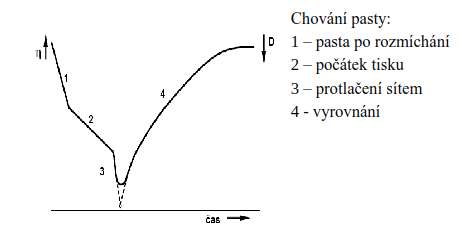
\includegraphics[width=0.6\textwidth]{viskozita.png}
      \caption{Časová závislost viskozity při nanášení pasty těrkou, mění se tedy tlak.}
      \label{fig:viskozita-png}
    \end{figure}
    

    \subsection{Zrnitost}
      Pasta je obvykle tvořena pevným práškem žádaného materiálu, rozptýleným v pojivu. Při práci s pastou musíme vzít v potaz velikost zrn v prášku. Ta by měla být pokud možno co nejvíce definovaná, stejně tak i tvar zrn. 
      Obvykle se pohybujeme v hodnotách od 1 do \qty{10}{\micro\meter}. Velikost zrn určuje mimo jiné také minimální tloušťku nátěru. 
      
      Určení velikosti zrn je možné za pomoci \textbf{grindometru}. Princip měření spočívá v rozetření pasty přes nakloněnou rovinu při konstantní výšce stěrky. V určitém bodě už zrna nevejdou do prostoru mezi rovinu a stěrku a jsou tedy setřeny pryč. Přístroj obsahuje stupnici, kde je možné následně odečíst požadovanou hodnotu velikosti zrn. 
	
% \section*{Reference}
% \printbibliography[heading=none]

% \clearpage

% \section*{Přílohy}

% \appendix % příkaz pro začátek sekce příloh
% \section{SPICE model \textbf{AD633} (ad633.lib)}
% \label{priloha:spicemodel}
% \lstinputlisting{../ad633.lib}

% \section{Ngspice kód pro simulace v~tomto projektu (projekt.cir)}
% \label{priloha:projekt.cir}
% \lstinputlisting{../projekt.cir}

% \(\) 
% \section{Výsledky fourierovy analýzy ve vlastním experimentu (\ref{sekce:vlastni-experiment})}
% \label{priloha:fourier-data}
% \subsection{\(f_{signal} =\)\qty{10}{\hertz}}
% \lstinputlisting{data/f/fourier_output10k+.txt}

% \subsection{\(f_{signal} =\)\qty{100}{\hertz}}
% \lstinputlisting{data/f/fourier_output100+.txt}

% \subsection{\(f_{signal} =\)\qty{1}{\kilo\hertz}}
% \lstinputlisting{data/f/fourier_output1k+.txt}

% \subsection{\(f_{signal} =\)\qty{10}{\kilo\hertz}}
% \lstinputlisting{data/f/fourier_output10+.txt}

% \subsection{\(f_{signal} =\)\qty{100}{\kilo\hertz}}
% \lstinputlisting{data/f/fourier_output100k+.txt}

\end{document}